
\chapter{Scenarios}

To allow researchers to evaluate learning agents in conditions of different characteristics, Vizia provides a mechanism of scenarios.

This chapter defines what a scenario is (see Section \ref{sec:scenario_definition}), describes sample scenarios provided with the API (see Section \ref{sec:scenarios}) and points out essentials of creating custom scenarios (see Section \ref{sec:creating_scenarios}).

\section{Definition}\label{sec:scenario_definition}
	Scenarios are DOOM resource files in special iwad format. A single scenario defines a map (structure of the world e.g. walls, corridors, monsters) and~a~script which determines behavior of entities and events. The script is also the place to assign rewards for various events. A scenario can define multiple maps in one iwad and~they all can be accessed by Vizia API. Default name for a map is `map01' but in general it can be completely arbitrary. Each map requires a separate script file.
	\\
	Scenarios cannot affect:
	\begin{itemize}
		\item constraints regarding buttons that can and cannot be used,
		\item episode timeout,
		\item skill level (they can affect; however, behaviors that depand on it),
		\item any rendering options e.g. screen resolution or~crosshair visibility,
		\item engine's reaction to player's death.
	\end{itemize}

	Due to scenarios' ability to set rewards they could be used to implement so called \emph{living~reward} and a~penalty for dying. Nonetheless, using API's \emph{setLivingReward} and \emph{setDeathPenalty} methods is the preferred way(see Section //TODO REF//) .

\section{Tools}\label{sec:tools}
	\begin{figure}
			\centering
			\includegraphics[scale=0.3]{slade.png}
			\caption{Slade 3 application for scenario creation.}\label{fig:slade}
	\end{figure}

	Creating iwad files involves compilation thus~requires dedicated software. \emph{Slade~3} and \emph{Doom~Builder~2} were the editors of choice because of huge popularity, availability of resources and~relative quality. The editors differ mostly in user interface details but~both provide most crucial functionalities:

	\begin{description}
		\item [Visual map editor] - a simple tool for map creation which is easy to use and~allows to build any imaginable map that Doom engine is capable of running.
		\item [Action Code Script support] - dedicated language resembling C that is suitable for determining behavior of any monster, player and~object in the game.
		\item [Testrunning] - possibility to test your scenario without leaving the editor. Test running requires providing a \emph{zdoom} executive file and \emph{doom2.wad} file (or~any other basic resource file) . 
	\end{description}

	Both tools are robust, reasonably easy to use and~provide much elasticity in sceanrio creation, although neither program is free from serious user experience shortcommings. Nevertheless, they still remain superior to other existing alternatives. Due to the lack of native \emph{Linux} support from \emph{Doom~Builder~2}, \emph{Slade~3} seems to be a more flexible solution. 

	\newpage
\section{Provided Scenarios}\label{sec:scenarios}
	This section describes ready-to-use scenarios that come with Vizia API.

	Each subsection includes `Suggested configuration' which suggests additional configuration which can be achieved by loading	configuration from a file or using additional API methods (see Section /REF/). These particular configurations are quite arbitrary and adjusting them to personal preferences is encouraged.

	\subsection{Basic}\label{subsec:basic}
		
		\begin{figure}
			\centering
			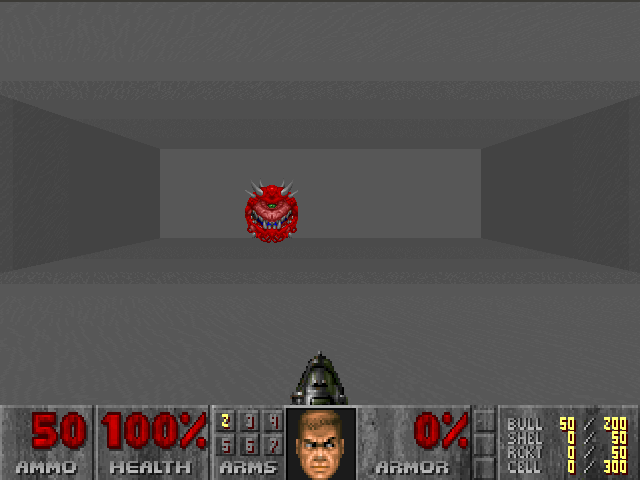
\includegraphics[scale=0.46]{basic.png}
			\caption{Doom gameplay frame from `basic' scenario.}\label{fig:basic}
		\end{figure}

		\paragraph{Motivation}
			Main purpose of this scenario is to show that using Vizia for Reinforcement Learning from visual input is a feasible idea. The scenario exposes most fundamental mechanics of the game like shooting, movement and delays between actions and reactions of the world.
		
		\paragraph{Decription}
			The map is a rectangle with gray walls, ceiling and floor. Agent is spawned along the longer wall, in the center. A red, circular monster is spawned randomly somewhere along the~opposite wall. Agent can only (config) move left, move right and~shoot. A single hit is enough to kill the~monster. Episode ends when the monster is killed or on timeout.
		
		\paragraph{Rewards}
			\begin{itemize}
				\item +101 for killing the monster
				\item -5 for missing
			\end{itemize}
		
		\paragraph{Suggested configuration}
			\begin{itemize}
				\item living reward = -1
				\item available buttons: move left, move right, shoot (attack)
				\item timeout = 300
			\end{itemize}
	\newpage

	\subsection{Deadly Corridor}
		\begin{figure}
			\centering
			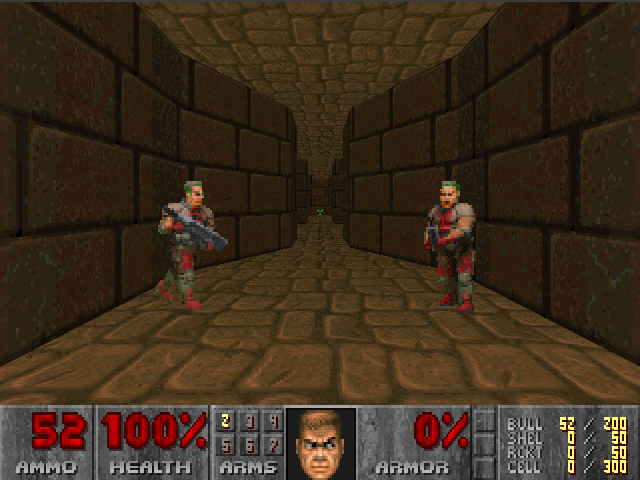
\includegraphics[scale=0.5]{deadly_corridor.png}
			\caption{Doom gameplay frame from `deadly corridor' scenario.}\label{fig:deadly_corridor}
		\end{figure}

		\paragraph{Motivation} 
			The purpose of this scenario is essentially to teach an agent to be a responsible adult with good spacial orientation: focus efforts towards a good direction and be able to sacrifice instant gratification in favour of future benefits and lifespan. Coping with the task requires some degree of spacial orientation and ability to see connection between monsters' presence and deteriorating health which, unattended, results in agent's death.

		\paragraph{Decription}
			The map is a corridor with shooting monsters along the longer walls (6 monsters in total). Agent is spawned at one end of the corridor and a green vest is placed at the oposite one. Reward is proportional (negative or positive) to change of the distance between the agent and the vest. If agent ignores monsters on the sides and runs straight for the vest he will be killed somewhere along the way. To ensure this behavior \textit{doom\_skill} equal to 5 (config) is needed.

		\paragraph{Rewards}
			\begin{itemize}
				\item $\Delta$x for getting closer to(further from) the vest by $\Delta$x units in the corridor's axis of symmetry.
			\end{itemize}
			
		\paragraph{Suggested configuration}
			\begin{itemize}
				\item available buttons: turn left, turn right, move left, move right, shoot (attack)
				\item timeout = 4200
				\item death penalty = 100
				\item doom skill = 5
				\item availale game variables: HEALTH
			\end{itemize}
	\newpage

	\subsection{Defend the Center}\label{subsec:defend_the_center}
		\begin{figure}
			\centering
			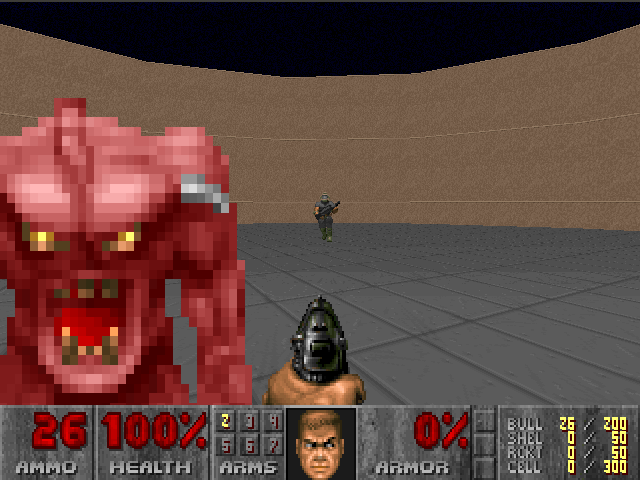
\includegraphics[scale=0.5]{defend_the_center.png}
			\caption{Doom gameplay frame from `defend the center' scenario.}\label{fig:defend_the_center}
		\end{figure}
		\paragraph{Motivation} 
			The purpose of this scenario is to encourage agents to develop some intuition about depth and awareness of potential dangers coming from behind. Obviously, agents should also learn that monsters are sinister and killing them is rewarding, but it is not sufficient. Coincidentaly an agent could be expected to learn to impersonate a classical Greek tragic hero: he is doomed to die pitifully (ammunition is finite) no matter his actions.

		\paragraph{Decription}
			The map is a large circle. Player is spawned in the exact center and is allowed to turn and shoot (config). 5 melee-only, monsters are spawned along the wall. Monsters are killed after a single hit. If slain, a monster is respawned after some time. Episode ends when the player dies (it's inevitable because of limitted ammunition supplies).

		\paragraph{Rewards}
			\begin{itemize}
				\item +1 for killing a monster
			\end{itemize}
		
		\paragraph{Suggested configuration}
			\begin{itemize}
				\item death penalty = 1
				\item available buttons: turn left, turn right, shoot (attack)
				\item available game variables: HEALTH, AMMO2(pistol ammo)
			\end{itemize}
	\newpage

	\subsection{Defend the Line}
		\begin{figure}
			\centering
			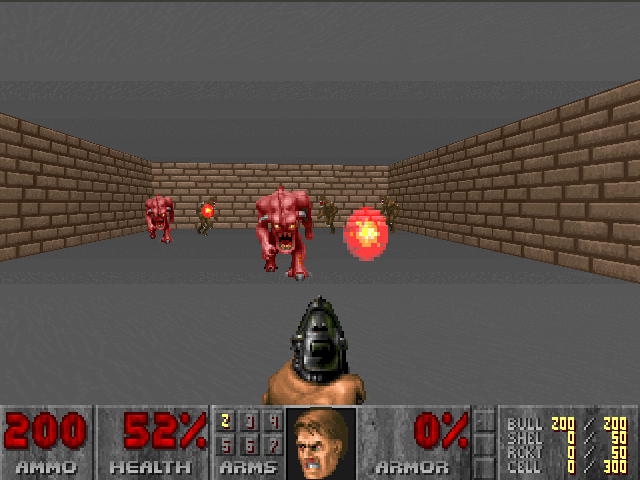
\includegraphics[scale=0.5]{defend_the_line.png}
			\caption{Doom gameplay frame from `defend the line' scenario.}\label{fig:defend_the_line}
		\end{figure}
		\paragraph{Motivation} 
			The purpose of this scenarios is to teach agents risk assessment and basic monster biology by presenting them with monsters of two types: melee and shoting. Agents should be able to recognize that shooters pose more imidiate threat than melee monster (unless they are at point blank range). Obviously, agents should also learn that monsters are sinister and killing them is rewarding, however it is not sufficient to perform superbly.
		\paragraph{Decription}
			The map is a rectangle. Player is spawned along the longer wall, in the center and is able to turn and shoot(config). 3 melee and 3 shooting monsters are spawned along the oposite wall. Monsters are killed after a single shot, at first. When slain, each monster is respawned after some time and can endure more damage than before. Episode ends when the player dies (it's inevitable because at some point monsters will be too tough to kill).
		\paragraph{Rewards}
			\begin{itemize}
				\item +1 for killing a monster
			\end{itemize}

		\paragraph{Suggested configuration}
			\begin{itemize}
				\item available buttons: move left, move right, shoot (attack)
				\item death penalty = 1
				\item available game variables: HEALTH, AMMO2(pistol ammo)
			\end{itemize}
	\newpage

	\subsection{Deathmatch}
		\begin{figure}
			\centering
			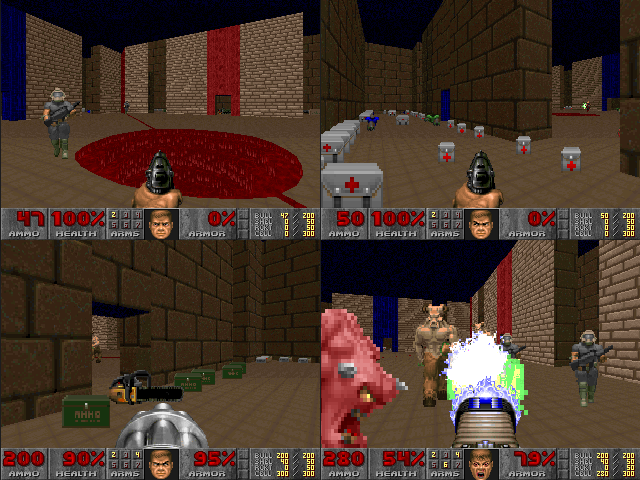
\includegraphics[scale=0.5]{deathmatch.png}
			\caption{4 Doom gameplay frames from `deathmatch' scenario.}\label{fig:deatchmatch}
		\end{figure}
		\paragraph{Motivation} 
	 		This scenario is a fully fledged fight for survival that hopefully requires quite sophisticated cognitive processess. Agent should be able to present effective understanding of many high level concepts as fleeing, surrounding awareness, hiding, camping, resupplying, navigation or changing weapons to survive and kill a signifficant number of monsters.

		\paragraph{Decription}
			The map consists of a square room (hall) of considerable size and 4 small rooms (supply rooms) adjacent to each wall of the hall. 2 supply rooms contain signifficant quantity of medkits and armours. Other 2 contain (each one) a shotgun, chainsaw, plasma gun, chaingun, rocket launcher and ammunition needed for aformentioned weapons. Agent is spawned in random location inside the hall. After a very short period monsters start spawning in random locations of the hall. Monsters include shooters and melee brawlers. Agent is rewarded for killing monsters. Toughest mosters are less probable to appear and produce greater rewards.
		\paragraph{Rewards}
			\begin{itemize}
				\item +1/2/3/4/5/10 for killing a monster (exact value depands on monster type).
			\end{itemize}
		
		\paragraph{Suggested configuration}
			\begin{itemize}
				\item available buttons: all buttons coresponding movement, turning, shooting and weapon change 
				\item timeout = preffered finite value
				\item death penalty = 100
				\item available game variables: HEALTH, ARMOR and all variables connected with weapons and ammo
			\end{itemize}		
	\newpage

	\subsection{Health Gathering}
		\begin{figure}
			\centering
			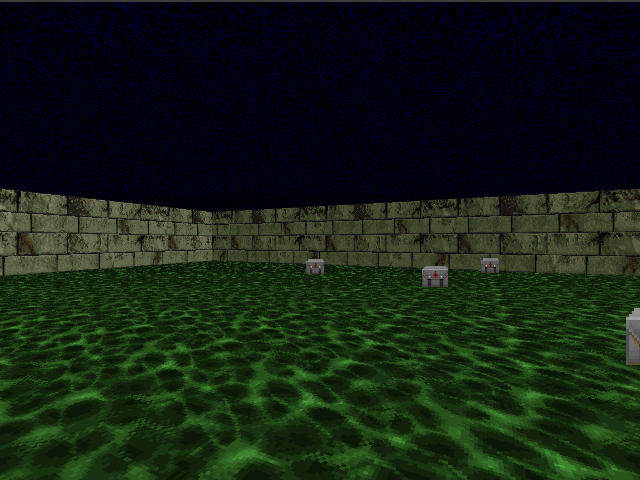
\includegraphics[scale=0.5]{health_gathering.png}
			\caption{Doom gameplay frame from `health gathering' scenario.}\label{fig:health_gathering}
		\end{figure}
		\paragraph{Motivation}
			The purpose of this scenario is to teach an agent that every second of his life is precious and collecting things increase his life expectancy in this brutal world. The agent should be able to see that deteriorating health causes death and how walking into medkits influences his health. It is advisable to equip the agent with some kind of memory because medkits that are directly in front of agent's feet cannot be noticed. In case of developing consciousness agent could also deduce that there is a devine being in the skies that loves him and sends medkits to save him.

		\paragraph{Decription}
			The map is a rectangle with green, acidic floor which hurts players periodically. Deadliness of acid depands on skill level. Agent is spawned in the exact center of the map and is able to turn and move forward (config).  Initially there are some medkits uniformly distributed over the map. New medkits fall from the skies peridically. A medkit heals some portion of player's health - to survive agent needs to pick them up. Episode finishes after player's death or on timeout.

		\paragraph{Suggested configuration}
		\begin{itemize}
			\item living reward = 1
			\item death penalty = 100
			\item available buttons: move left, move right, move forward
			\item timeout = 2100
			\item available game variable: HEALTH
		\end{itemize}
	\newpage

	\subsection{My Way Home}
		\begin{figure}
			\centering
			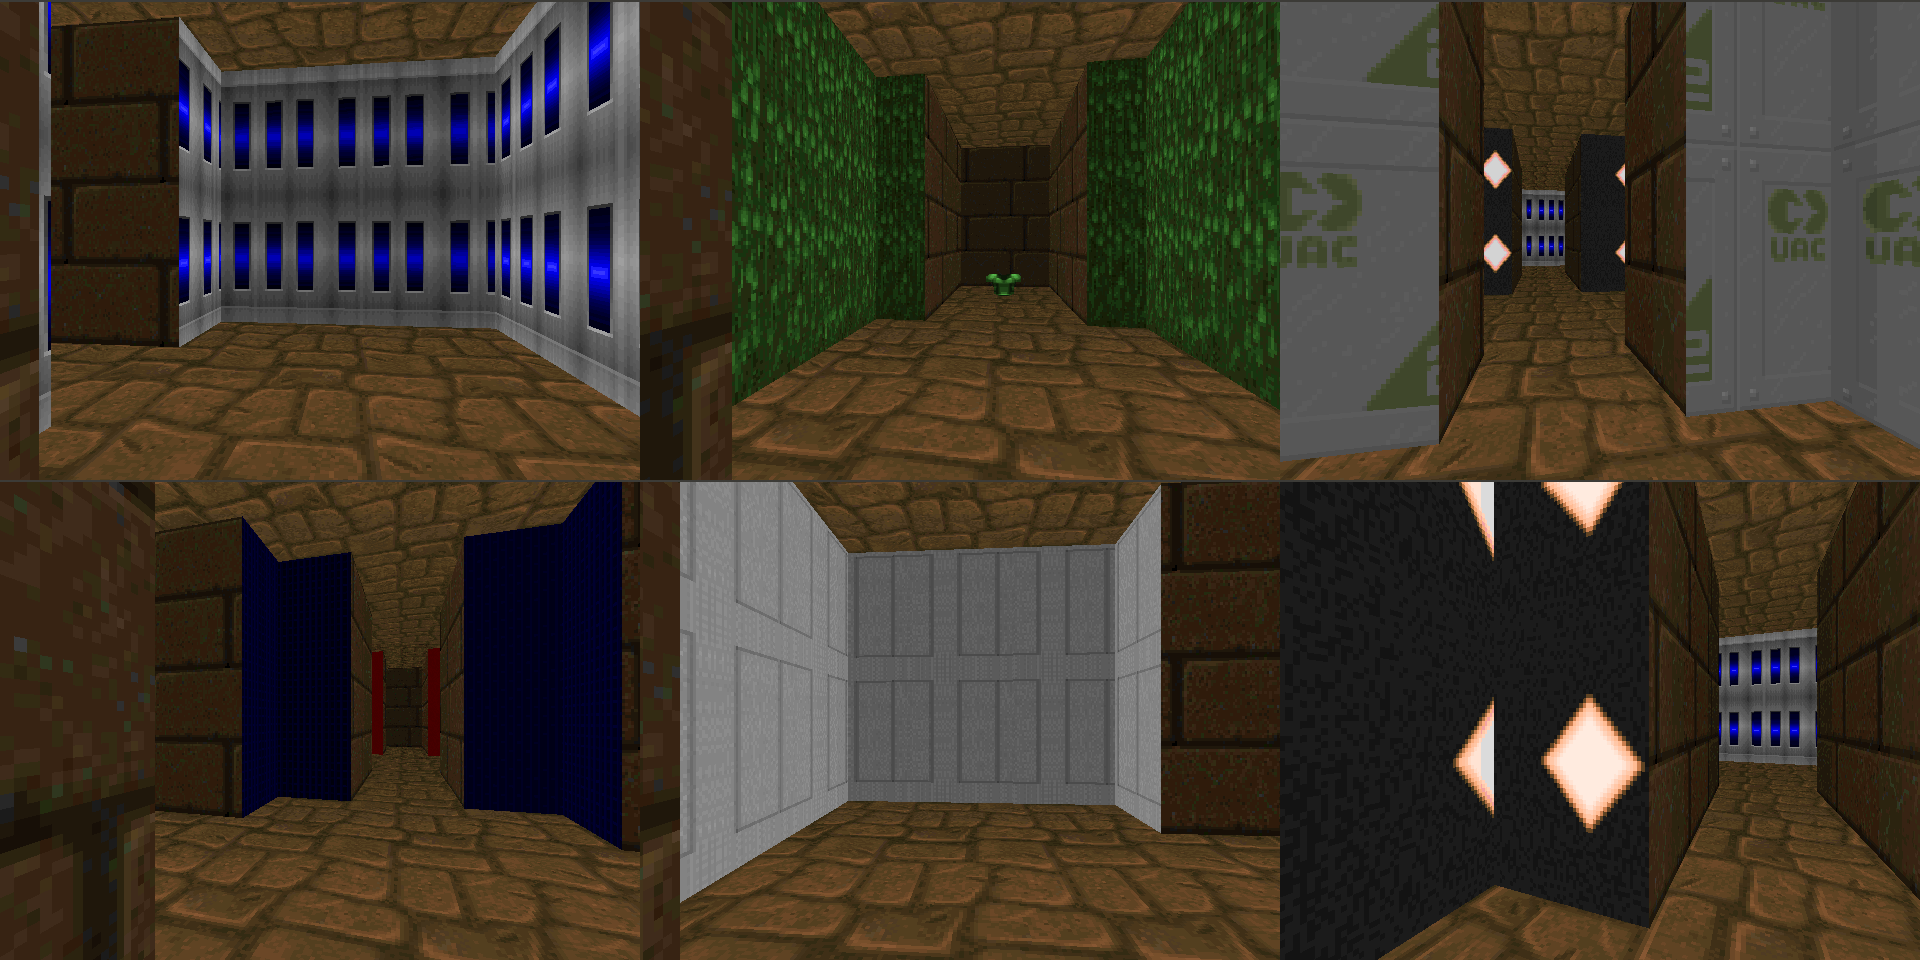
\includegraphics[scale=0.22]{my_way_home.png}
			\caption{6 Doom gameplay frames from `my way home' scenario.}\label{fig:my_way_home}
		\end{figure}
		\paragraph{Motivation} 
			The purpose of this scenario is to teach the agent how to navigate in a labirynth-like surroundings and reach his ultimate goal (and learn what the goal actually is). Agent should learn to determine his position in the maze and to navigate.

		\paragraph{Decription}
			The map is a series of small rooms interconnected with each other by short passages and a single dead end corridor. Each room has a different color. A green vest is placed in one of the rooms (the same room every time). Player is spawned in randomly choosen room facing a random direction. Episode ends when the vest is reached or on timeout.
		\paragraph{Rewards}

		\begin{itemize}
			\item +1 for reaching the vest
		\end{itemize}
		
		\paragraph{Suggested configuration}
		\begin{itemize}
			\item living reward = -0.0001
			\item available buttons: move left, move right, shoot (attack)
			\item timeout = 2100
		\end{itemize}
	\newpage

	\subsection{Predict Position}
		\begin{figure}
			\centering
			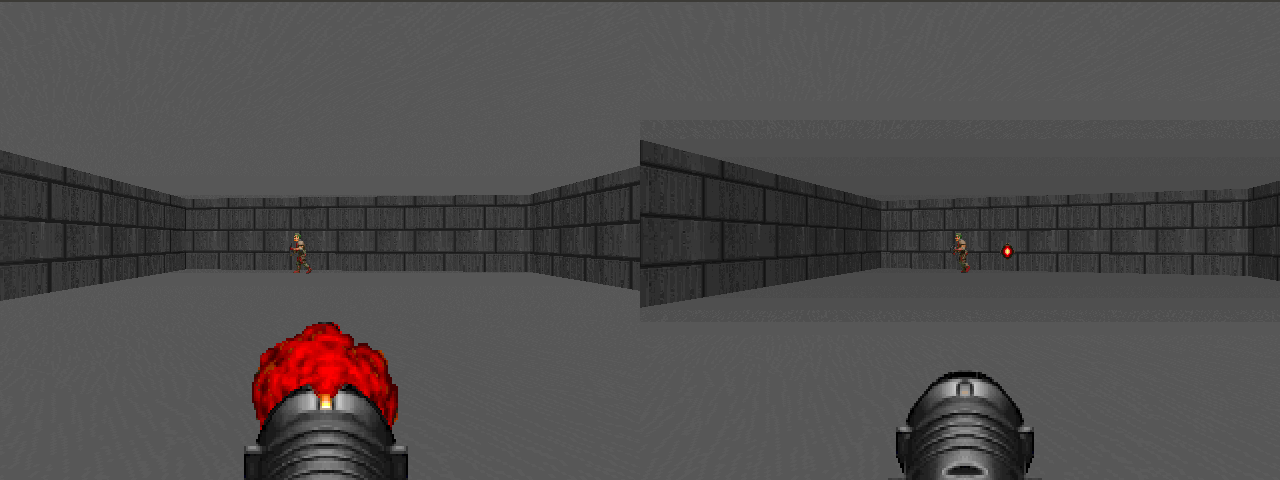
\includegraphics[scale=0.32]{predict_position.png}
			\caption{2 Doom gameplay frames from `predict position' scenario.}\label{fig:predict_position}
		\end{figure}
		\paragraph{Motivation} 
			The purpose of the scenario is to teach agents to synchronize missle weapon shots (involving a signifficant delay between shooting and hitting) with target movements. Agent should be able to shoot so that missle and monster meet each other.

		\paragraph{Decription}
			The map is a rectangle room. Agent is spawned along the longer wall, in the center and is allowed to turn and shoot(config). A monster is spawned randomly somewhere along the opposite wall and walks between left and right corners along the wall. Player is equipped with a rocket launcher and a single rocket. Episode ends when the missle hits the monster (or a wall) or on timeout.
		\paragraph{Rewards}
		\begin{itemize}
			\item +1 for killing the monster
		\end{itemize}
		
		\paragraph{Suggested configuration}
		\begin{itemize}
			\item living reward =-0.0001
			\item available buttons: turn left, turn right, shoot (attack)
			\item timeout = 300
		\end{itemize}
	\newpage

	\subsection{Take Cover}
		\begin{figure}
			\centering
			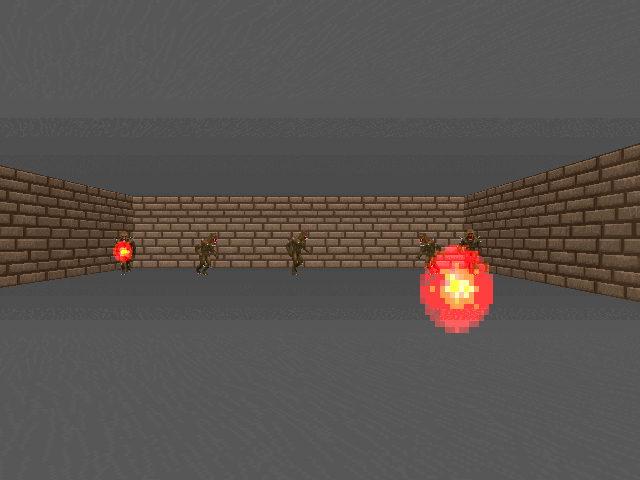
\includegraphics[scale=0.5]{take_cover.png}
			\caption{Doom gameplay frame from `take cover' scenario.}
		\end{figure}
		\paragraph{Motivation} 
			The purpose of this scenario is to teach agents to link incomming missles with their estimated lifespan. Agents should learn that being hit means a decrease in health and this in turn leads to death that is most undesirable. In effect agents should learn how to avoid missles.

		\paragraph{Decription}
			Map is a rectangle. Player is spawned along the longer wall, in the center. A couple of fireball-spitting monsters are spawned randomly somewhere along the opposite wall and try to kill the player with fireballs. The player has no weapon and can only move sideways (config). More monsters appear with time. Episode ends when player dies which is inevitable.

		\paragraph{Suggested configuration}
		\begin{itemize}
			\item living reward = 1
			\item death penalty = 100
			\item 2 available buttons: move left, move right
		\end{itemize}
	\newpage


\section{Creating scenarios}\label{sec:creating_scenarios}
	This section is not intended as a reference manual for Action Code Script (ACS) or map creation thus covers only subjects directly relevant to interfacing between Doom game engine and Vizia API.


	\subsection{Fixed Point Numbers}\label{subsec:fixed_point}
		ACS does not support floating point numbers. However, fixed point numbers are implemented with integers. By adding a decimal point you force compiler to treat it as a fixed point number so for instance `1' will be treated as an integer whereas `1.0' as a fixed point numeral. Mixing integers and fixed point numbers is allowed but will produce unexpected results if performed unknowingly. For more detailed information consult ZDOOM Wiki //TODO REFERENCE

	\subsection{Global Variables}\label{subsec:global_variable}
		ACS, except from ordinary variables, provide global variables which can be accessed by Vizia api as user variables (see //TODO REF TO API//). Global variables behave the same as ordinary variables but need to be declared in global scope and in a slightly different way:
		\begin{clinee}
global int <X>:reward;
		\end{clinee}
		Where <X> denotes the ordinal number of the variable.
		
	\subsection{Rewards}
		In order to support rewarding mechanism, it is neccessary to utilize global variable 0 in ACS script. Name given to the variable does not matter. Value of the variable represents total reward accumulated throughout whole episode so in order to give reward for specific action you need to increase global variable 0 by the desired value not assign it. Vizia will treat the variable as a fixed point number(see \ref{subsec:fixed_point}).

	\subsection{Advices}
		This section shows code snippets showing how we achive some ACS scripting behaviors that may prove useful. The code snippets intend to be relatively self-explanatory and assume knowledge of the very basics of ACS scripting and capability of reading documentation to make sense of used functions. For documentation and more detailed information consult ZDOOM Wiki //TODO REFERENCE

		\subsubsection*{Ending an Episode}

			\begin{clinee}
Exit_Normal(0);
			\end{clinee}
		\subsubsection*{Reward for Killing a Monster} This snippet is also useful for triggering any event after killing a monster or collecting an item.
			\begin{clinee}
script 123 (void)
{
	reward = reward + 1;
}
SetThingSpecial(MONSTER_TID, ACS_ExecuteAlways, 123);
			\end{clinee}
\subsubsection*{Friendly Monster}
			\begin{clinee}
Thing_Hate (MONSTER_TID, SOME_UNUSED_TID, 6);
			\end{clinee}
		\subsubsection*{Stationary Monster}
			\begin{clinee}
SetActorProperty(MONSTER_TID, APROP_Speed, 0);
			\end{clinee}
		\subsubsection*{Single Hit Monster}
			\begin{clinee}
SetActorProperty(MONSTER_TID, APROP_Health, 1);
			\end{clinee}
		\subsubsection*{Self-replenishing Ammo}
		Note that this can also be achieved by changing Zdoom's configuration but is persistent.
			\begin{clinee}
script 2 ENTER
{   
    while(1)
    {
        delay(1);
        GiveInventory("Clip", 1 );
    }
}
			\end{clinee}
		\subsubsection*{Disappearing Corpses}
			\begin{clinee}
script 234 (int TID)
{
	Thing_Remove(TID);
}
SetThingSpecial(MONSTER_TID, ACS_ExecuteAlways, 234, MONSTER_TID);
			\end{clinee}
